\subsection*{Kategorisering}
Kategorisering inddeles i fire boundarys og en dertilhørende controlklasse, som det fremgår af \autoref{fig:DesignKategorisering}.

\begin{figure} [H]
\centering
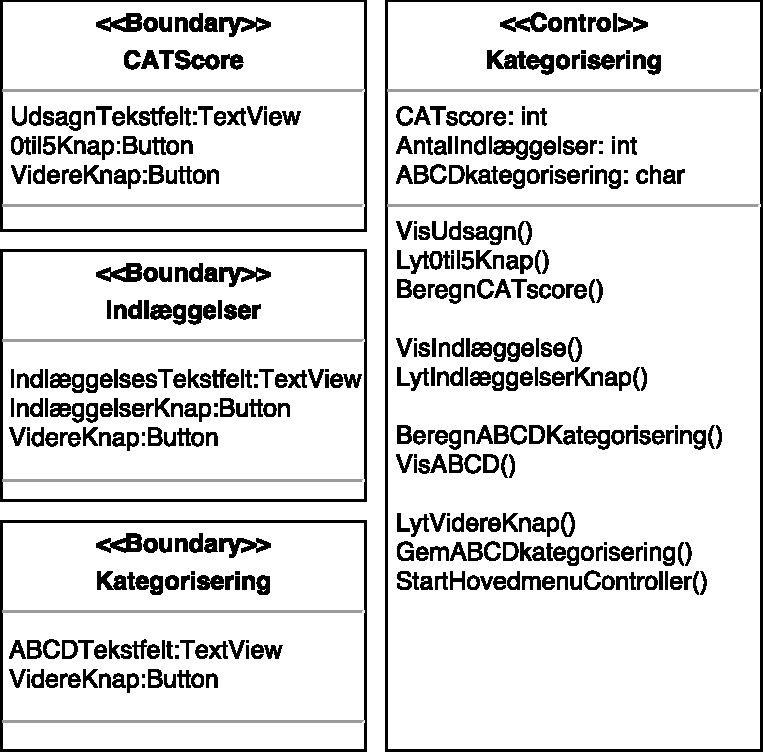
\includegraphics[width=1\textwidth]{figures/MVC/MVCKategorisering}
\caption{Designklasser for kategorisering. Til venstre ses de forskellige grænseflader, henholdsvis Introduktion, CATscore, Indlæggelser og Kategorisering. Til højre fremgår den dertilhørende controller.}
\label{fig:DesignKategorisering}
\end{figure}

\noindent
Kategoriseringen inddeles i fire grænseflader, herunder \textit{Introduktion}, \textit{CATscore}, \textit{Indlæggelser} samt \textit{Kategorisering}. Dette er valgt, idet grænsefladerne skal have forskellige layouts, og en opdeling vil gøre implementeringen af grænsefladerne mere overskuelig. Desuden ønskes det at gøre app’en brugervenlig, hvilket kan opnås ved at tydeliggøre adskillelsen mellem CATscore og besvarelse af antal årlige indlæggelser, jf. gestaltloven om lighed i \autoref{sec:brugervenlighed}. Hertil skal brugeren foretage minimale valg på hver grænseflade, således
brugeren ikke eksponeres til for mange valg på samme tid samt informationer på én grænseflade.

De fire grænseflader indeholder tekstfelter af typen TextView, der informerer brugeren om den følgende handling, brugeren skal foretage. Dertil er der ligeledes opsat knapper af typen Button, således brugeren kan besvare udsagn. I boundaryklassen \textit{CATscore} ses 0til5Knap, som repræsenterer seks forskellige knapper, der skal implementeres i grænsefladen. Disse seks knapper vil gøre det muligt for brugeren at vælge en værdi mellem 0 og 5 for hvert udsagn. Ligeledes ses der i boundaryklassen \textit{Indlæggelser} en knap, IndlæggelserKnap, som repræsenterer to knapper i grænsefladen. Brugeren skal på denne grænseflade angive antallet af årlige indlæggelser på grund af KOL, hvor knapperne gør det muligt at vælge mellem ingen eller flere indlæggelser.

Den dertilhørende controller, \textit{Kategorisering}, håndterer visningen af de fire boundarys samt respektive knapper og tekst. Attributterne for denne controller er private. En af disse fremgår som et ArrayList, der er et array, som anvendes til beregning af CATscore. Controlleren indeholder ligeledes private metoder Vis, Lyt, Beregn, Send og Start, som handler i forhold til de definerede inputsparametre. BeregnKategorisering returnerer dertil en kategorisering af typen string, således denne senere kan sendes og gemmes i databasen. Der er ligeledes udarbejdet et sekvensdiagram for kategorisering, hvilket ses af \autoref{fig:SEKKategorisering}.

\begin{figure} [H]
\centering
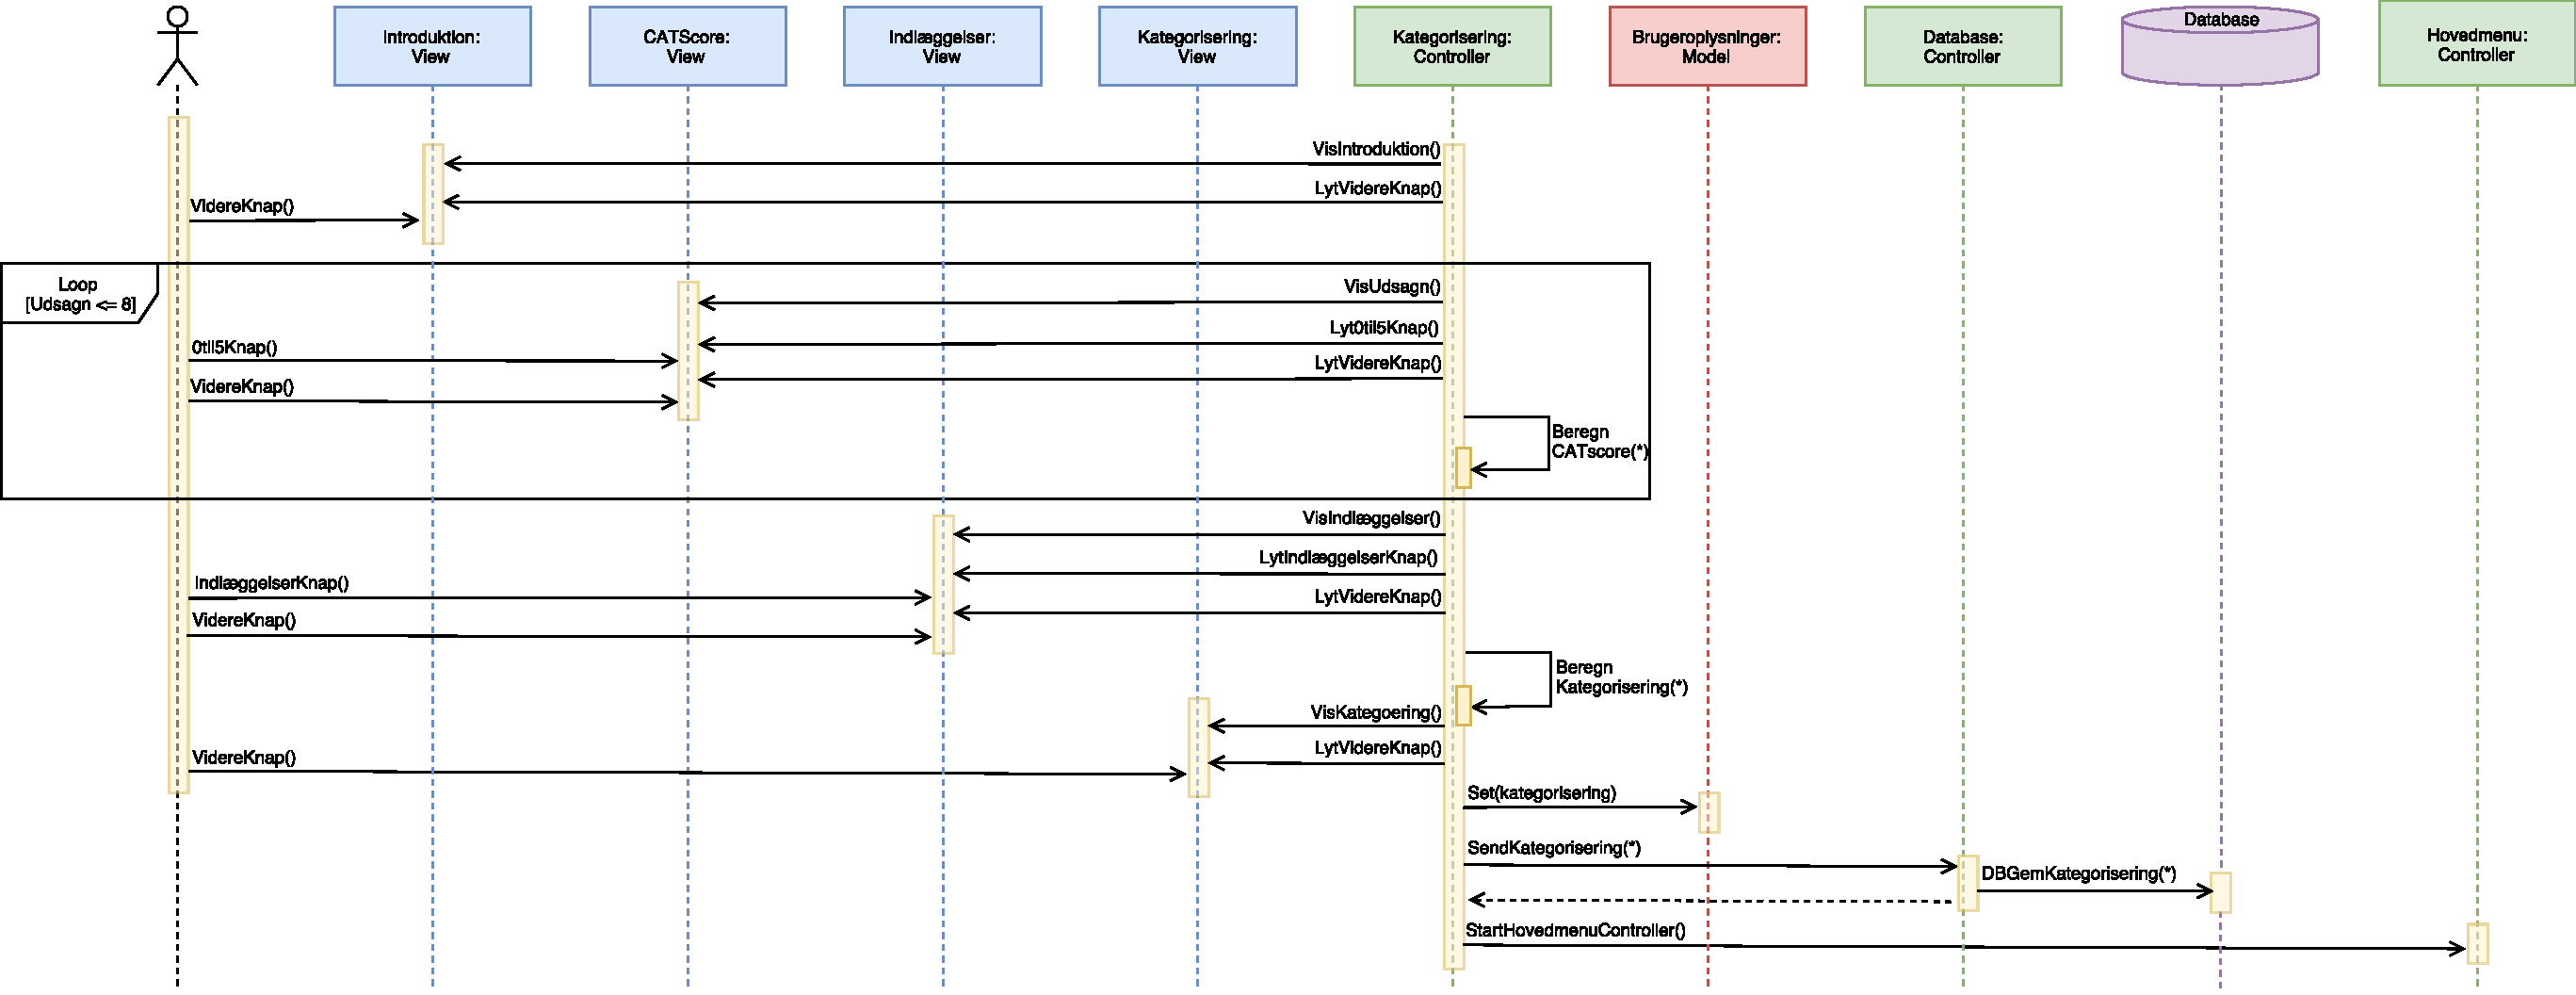
\includegraphics[width=1.55\textwidth, angle=90]{figures/Sek/SEKKategorisering}
\caption{Sekvensdiagram for kategorisering.}
\label{fig:SEKKategorisering}
\end{figure}

\noindent
Det fremgår af sekvensdiagrammet, at grænsefladen for \textit{Introduktion} vises som det første. Denne grænseflade skal informere brugeren om kategoriseringen, der skal foretages for således, at træningsniveau kan tilpasses. Idet brugeren trykker på VidereKnap vises de otte udsagn, der er opstillet i et loop. Udsagnene besvares ved hjælp af knapper fra 0 til 5. Idet brugeren trykker videre fra hvert udsagn, adderes CATscoren. Efter de otte udsagn er besvaret, og den samlede CATscore er beregnet, vises grænsefladen for \textit{Indlæggelser}. Stjerner angivet i parenteser angiver inputsparametre, som er beskrevet i tilhørende designklasser.


Controlleren lytter dertil til IndlæggelserKnap, hvori brugeren besvarer antal årlige indlæggelser forårsaget af KOL. Besvarelsen bekræftes ved at benytte videreKnappen. Kategoriseringen kan derved beregnes og vises i \textit{Kategorisering} grænsefladen. Denne kategorisering gemmes i entityen \textit{Brugeroplysninger} og sendes til controlleren for \textit{database}, hvorved denne gemmer kategoriseringen i \textit{database}. Herefter startes \textit{hovedmenu} controlleren. 
